%========================================
%% Minimun Test File
%% Encoding: UTF-8
%% HOW TO RUN: xelatex test.tex
%% 正确的PDF编译结果:
% 显示4幅图像,分别是EPS,PDF,PNG,JPG格式
% 显示"中文测试"和英文内容
% 嵌入AdobeSongStd和NimbusRomNo9字体(通过PDF阅读器的“属性”查看)
% 英文字符正确连字(ligature)
% textsc正确工作
%========================================


\documentclass[12pt,a4paper,UTF8,adobefonts]{ctexbook}

% AMS math
\RequirePackage{amsmath,amsthm,amsfonts,amssymb,bm,mathrsfs} 

% Font Setting
\usepackage{fontspec}
\RequirePackage{xltxtra} % \XeTeX Logo
\setmainfont{TeX Gyre Termes} % an SC-capable OTF font that looks like Times
\renewcommand\labelitemi{\ensuremath{\bullet}} % 原来定义为 \textbullet

% Graph
\usepackage{graphicx}
\usepackage{subfigure}
\usepackage{ccaption}
% 设置图形文件的搜索路径
\graphicspath{{figure/}{figures/}{logo/}{logos/}{graph/}{graphs}}
% 如果插入的图片没有指定扩展名,那么依次搜索下面的扩展名所对应的文件
\DeclareGraphicsExtensions{.pdf,.eps,.png,.jpg,.jpeg}
% 重定义\nobreakspace命令
\DeclareRobustCommand\nobreakspace{\leavevmode\nobreak\ }

\begin{document}

中文测试 TeX Gyre Termes ff fi fl ffi \textsc{PostScript} % 检查连字

\begin{displaymath}
  E=mc^2 \quad \mathscr{ABCDE abcde 1234} \quad \mathfrak{ABCDE abcde 1234} \quad \mathbb{ABCDE abcde 1234}
\end{displaymath}

\begin{figure}
  \centering
  \subfigure[EPS Figure]{
    \label{fig:demo:a} %% label for first subfigure
    \includegraphics[width=0.3\textwidth]{chap2/testeps}}
  \hspace{1in}
  \subfigure[PDF Figure]{
    \label{fig:demo:b} %% label for second subfigure
    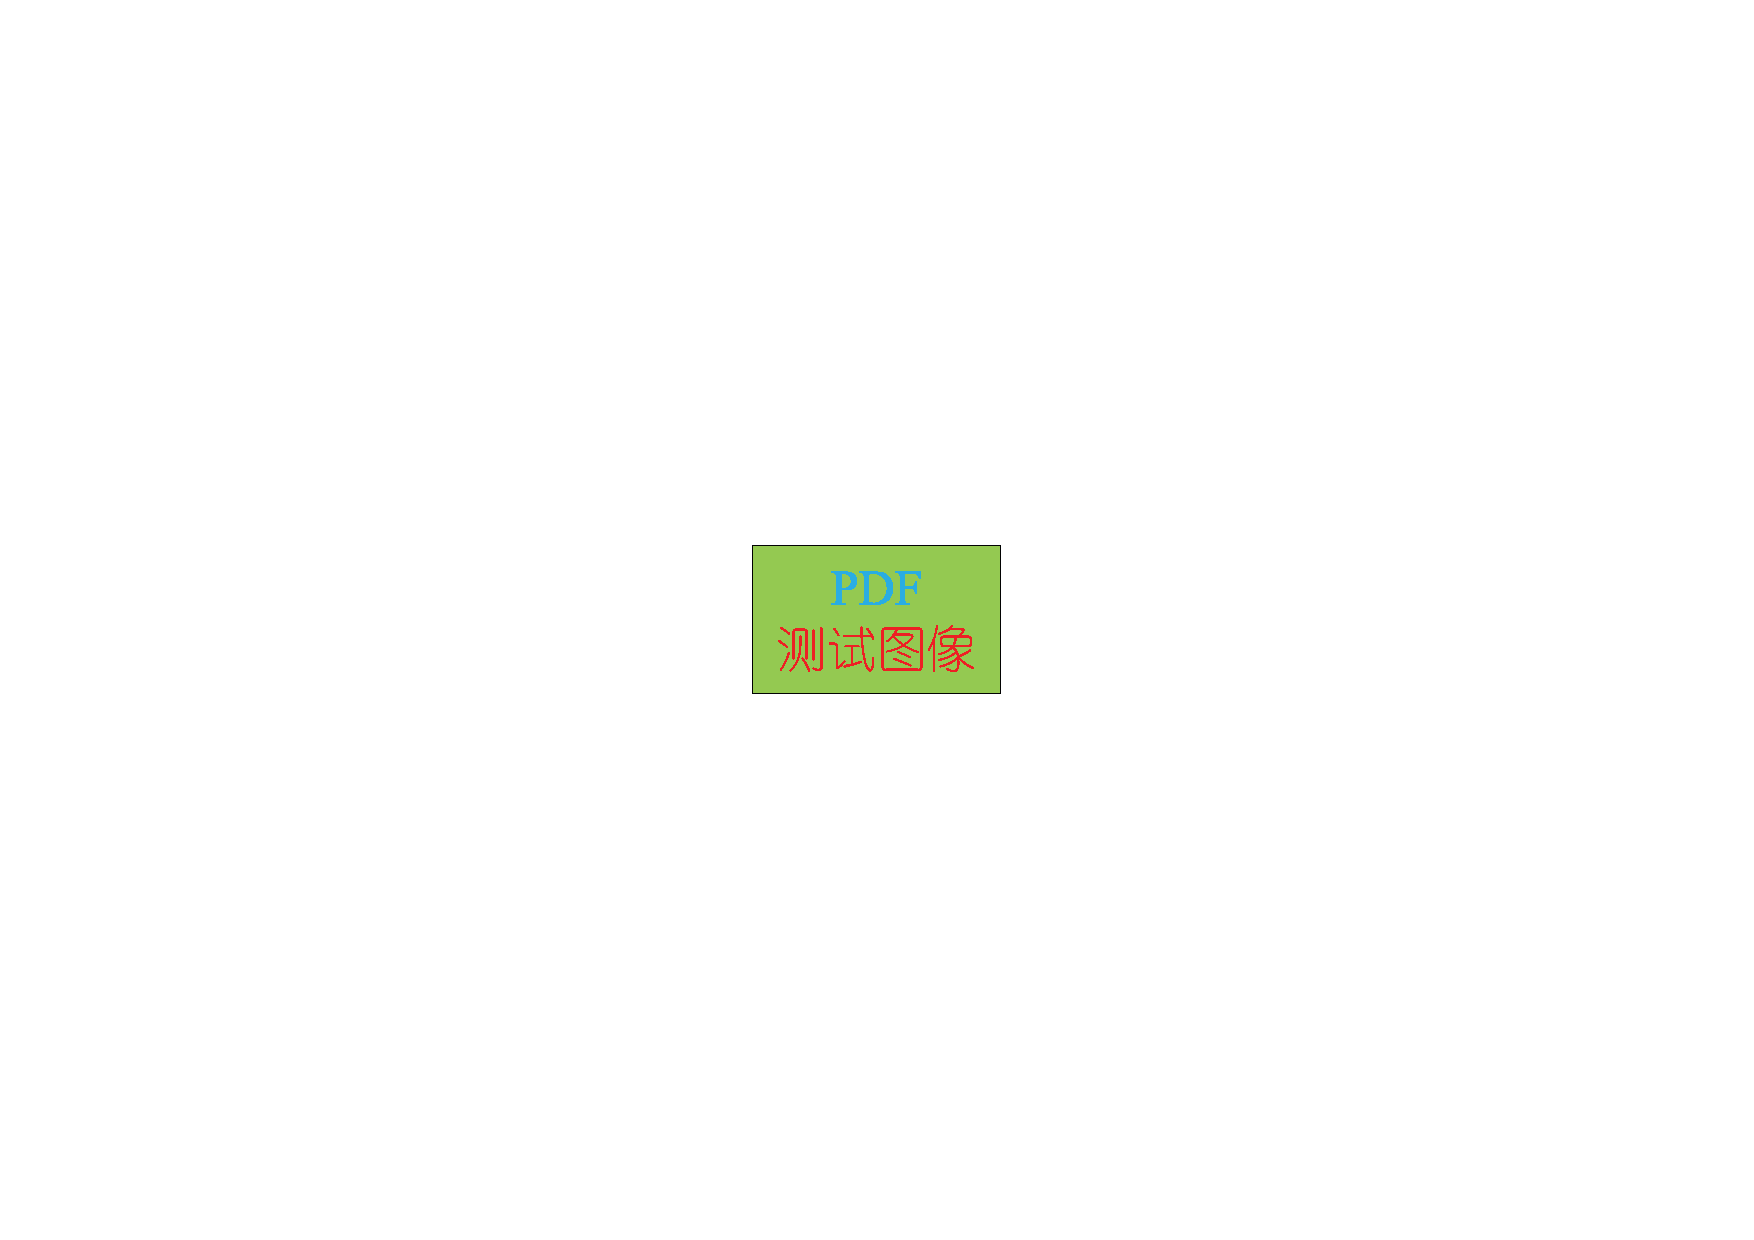
\includegraphics[angle=-90,origin=br,width=0.3\textwidth]{chap2/testpdf}}
  \\ % newline
  \subfigure[PNG Figure]{
    \label{fig:demo:c} %% label for third subfigure
    
\includegraphics[width=0.3\textwidth]{chap2/testpng}}
  \hspace{1in}
  \subfigure[JPG Figure]{
    \label{fig:demo:d} %% label for fourth subfigure
    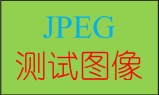
\includegraphics[width=0.3\textwidth]{chap2/testjpg}}
  \bicaption[fig:demo]{插入图像}{插入图像的例子}{Fig}{A demo}
\end{figure}

\begin{itemize}
\item Hello
\item World
\end{itemize}

\section{一段测试文字}

  上海交通大学是我国历史最悠久的高等学府之一,是教育部直属、教育部与上海市共建的全国重点大学,是国家 “七五”、“八五”重点建设和“211工程”、“985工程”的首批建设高校。经过115年的不懈努力,上海交通大学已经成为一所“综合性、研究型、国际化”的国内一流、国际知名大学,并正在向世界一流大学稳步迈进。 


\end{document}
